Проведем анализ производительности полученных версий анализатора. В качестве
данных для тестирования возьмем выражения вида $\underbrace{2 + 2 + 2 \dots +
2}_{n}$ для $n = 1\dots100$ с шагом $1$. Для вычисления времени выполнения
воспользуемся библиотекой \verb|time| Python 3.9.5. Автоматизацию обеспечим с
помощью библиотеки \verb|subprocess|. Получим следующий код:

\inputminted{python}{test.py}

Кроме того, отметим, что в ранее написанные программы были внесены некоторые
изменения для проведения эксперимента. Ознакомиться с ними можно в приложении А.

Ознакомиться с полным исходным кодом программы, осуществляющей исследование
производительности можно в приложении Б.

Для большей наглядности графики интерполированы полиномом с помощью функции
\verb|polyfit| библиотеки \verb|numpy|.

Ознакомиться с полным исходным кодом программы, осуществляющей анализ полученных
результатов можно в приложении В.

Результаты исследования изображены на рис. 2:

\begin{figure}[hbt!]
    \centering
    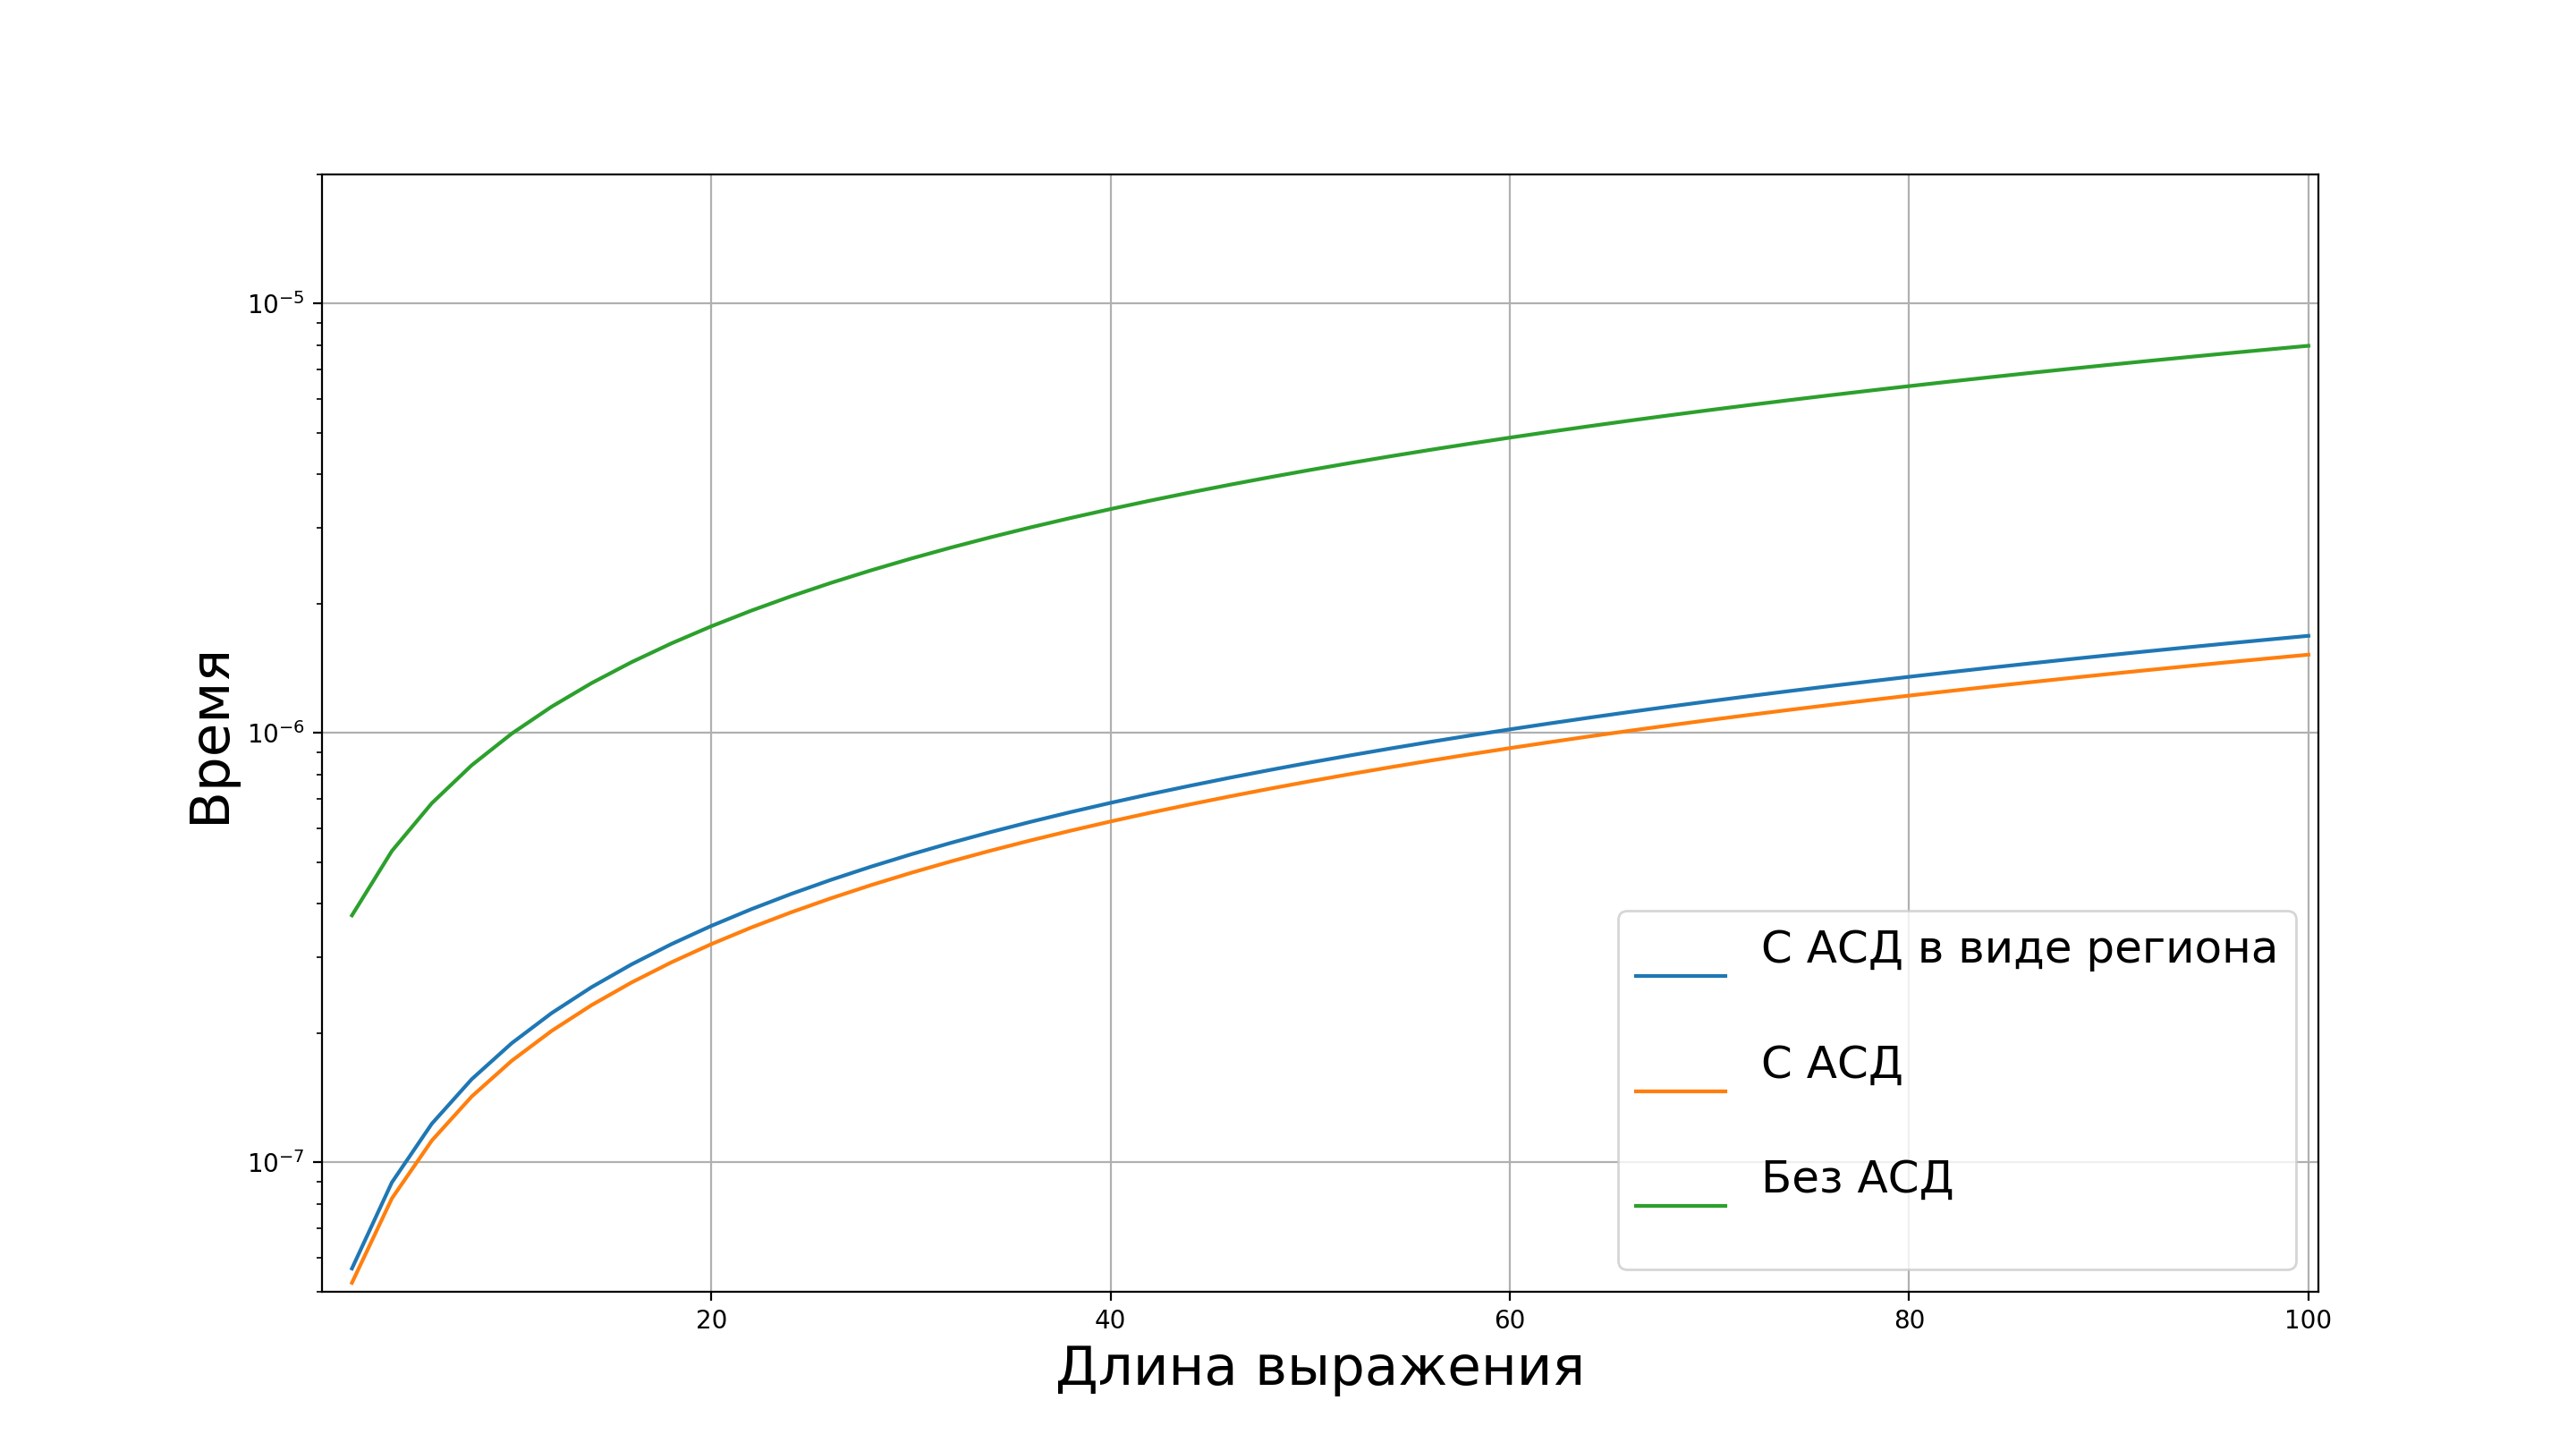
\includegraphics[scale=0.5]{benchmark.png}
    \caption{Сравнение полученных результатов}
    \label{fig:benchmark}
\end{figure}

Исследование показало, что использование абстрактных синтаксических деревьев
позволяет уменьшить время работы программы более чем в $5$ раз, что существенно
заметно для выражений любой длины.

Также из графиков видно, что в рамках данной работы не удалось добиться большей
производительности при управлении памятью на основе регионов. Тем не менее, она
все еще может считаться более предпочительной ввиду перечисленных ранее
преимуществ.